
\chapter{Návrh nástroje pro penetrační testování}
Pro detekování chyb typu SQL Injection je v této části vysvětlen postup a princip fungování nástroje pro penetrační testování. V další části 5.1 je uveden detailně postup od zpracování webové stránky až po metody testování a rozpoznání SQL Injection chyby.

\section{Postup testu}
\begin{enumerate}
\item Analýza zdrojového kódu 
\begin{itemize}
\item Získání objektové reprezentace webové stránky použitelné pro další zpracování.
\end{itemize}
\item Vytvoření stromu webové stránky
\begin{itemize}
\item Extrahování formulářů a hypertextových odkazů z webové stránky (pro vytvoření stromu).
\item Normalizace URL adres kvůli detekování přechodu na jiné domény a sjednocení všech možných kombinací relativních a absolutních URL adres.
\end{itemize}
\item Otestování hypertextových odkazů
\begin{itemize}
\item Otestování možnosti SQLi v hypertextových odkazech pomocí analýzy webové stránky (změna stránky - počtu elementů v závislosti na úpravě sql dotazu).
\end{itemize}
\item Otestování formulářů
\begin{itemize}
\item Stejný postup jako u hypertextových odkazů.
\end{itemize}
\item Reprezentace výsledků
\begin{itemize}
\item Reprezentace výsledků pro další zpracování - na standardní výstup, popřípadě ve specifickém formátu do souboru.
\end{itemize}
\end{enumerate}

\section{Analýza zdrojového kódu stránky}
Při analýze stojí za úvahu, zda si napsat vlastní HTML parser nebo použít nějaký stávající, čímž by bylo rozhodnuto i o jazyce, ve kterém bude testovací skript napsán. Bylo možné použít  následující HTML parsery:
\begin{itemize}
\item XML Reader - PHP
\item Simple HTML DOM - PHP
\item Nokogiri - Ruby
\item Hpricot - Ruby
\item JSoup - Java
\end{itemize}

\subsection{Testování parserů}
Pro testování jsem si napsal 2 webové stránky, první s validním a správně napsaným HTML a druhou s rozházenými tagy, nedokončenými uvozovkami, která by měla více reprezentovat reálný model webových stránek. I když existují xHTML standardy je většina projektů psaná \uv{ve spěchu} a kód bývá dost často nepořádný. Proto je nutné tento problémem zohlednit.\\
\newline
\textbf{XML Reader - PHP} - Tento parser je primárně pro parsování validních XML dokumentů, proto se ukázal pro parsování HTML stránek jako nevhodný.\\
\textit{(Ke stažení na: http://php.net/manual/en/book.xmlreader.php)}\\
\newline
\textbf{Simple HTML DOM - PHP} - Parser v PHP určený přímo pro parsování HTML DOM Modelu se jevil jako vhodný kandidát, ale při otestování na reálném webu (sestavování stromu webové stránky) se parser ukázal jako nepoužitelný. Velmi špatně reagoval na další chyby v HTML stránce a nebylo možné je rozumně zachytávat. Také jeho výběr prvků a následné parsování dat bylo nutné kombinovat s regulárními výrazy. Ze zmíněných důvodů jsem od tohoto parseru upustil.\\
\textit{(Ke stažení na: http://simplehtmldom.sourceforge.net/)}\\
\newline
\textbf{Nokogiri - Ruby} - První parser v testu, který si bez problémů poradil s parsováním špatných HTML stránek, byl schopen rozpoznat správně odkazy, chybné uzavírání parametrů. Další obrovským přínosem je, že funguje na principu CSS3 selektorů:
\begin{lstlisting}[label=rubyNokogiriSelections,language=Ruby, caption=CSS3 Selektory NokoGiri]
# Load Nokogiri::HTML Document for page
doc = Nokogiri::HTML(open('http://www.google.com/search?q=sparklemotion'))

# Search for nodes by css
doc.css("body a").each do |link|
	puts link.content
end
\end{lstlisting}
Dále implementuje XPath a elementy dále rozděluje (ne jako předchozí parser Simple HTML DOM, který vrací pouze textovou podobu).
\begin{lstlisting}[label=rubyparser,language=Ruby, caption=Parsování]
# Search for nodes by css
doc.css("body a").each do |link|
	puts link['href'] # Print href attribute
end
\end{lstlisting}
\textit{(Ke stažení na: http://nokogiri.org/)}\\
\newline
\textbf{HPricot - Ruby} - Další parser v Ruby, který je hodně podobný předchozímu Nokogiri. Opět si poradí s CSS3 selektory, Xpath výrazy atd. Má jedinou nevýhodu: není již dále vyvíjen a podporován.\\
\textit{(Ke stažení na: https://github.com/hpricot/hpricot/)}\\
\newline
\textbf{JSoup - Java} - První HTML parser, který je napsán v programovacím jazyce Java. Podporuje XPath, ale pouze CSS selektory. Největší nevýhodou je samotný programovací jazyk. Vývoj v Javě je zdlouhavý, a proto jsem volil rychlejší programovací jazyky, kterým je Ruby a PHP. Další nevýhodou Javy je, že není možná integrace do Metasploit frameworku (o Metasploitu viz kapitola 2.6), který je napsán v Ruby.\\
\textit{(Ke stažení na: http://jsoup.org/)}

\subsection{Závěr testu parserů}
Každý z testovaných parserů měl své výhody a nevýhody, nicméně z testů vyšel jednoznačně nejlépe parser \textit{Nokogiri}, který určil i programovací jazyk, ve kterém penetrační test bude napsán - \textit{Ruby ve verzi 1.9.3}. 

\section{Vytváření stromu webových stránek}
Abychom mohli získat všechny odkazy a formuláře na webových stránkách, musíme určit URL strom (viz obrázku \ref{obr.url_stack}) a z něj následně získat všechny odkazy a formuláře.
\begin{figure}[h!]
\centering{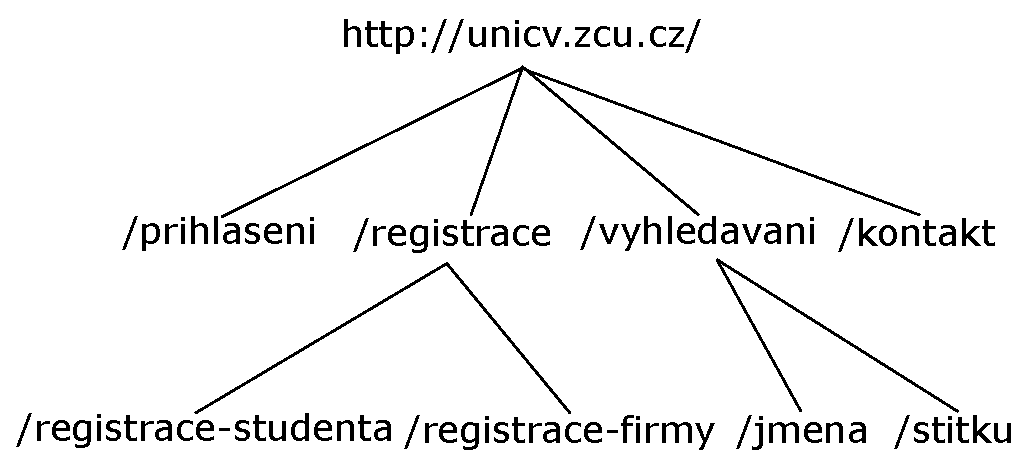
\includegraphics[width=200px]{url_tree.eps}}
\caption{Ukázka stromu webových stránek}
\label{obr.url_stack}
\end{figure}
Získávání stromu je postaveno na strukturách zásobník a datové pole. V zásobníku se ukládají URL pro další provádění a úroveň zanoření (je možné pomocí parametru \textit{-l N}, kde N je hloubka zanoření, definovat, do jaké \uv{hloubky}, se budou odkazy prohledávat). Na referenčním obrázku \ref{obr.url_stack} vidíme, že zanoření úrovně 0 je stránka \textit{http://unicv.zcu.cz}, zanoření úrovně 1 jsou podstránky \textit{/prihlaseni, /registrace, /vyhledavani, /kontakt} a tak dále.

\subsection{Funkce zásobníku}
\begin{figure}[h!]
\centering{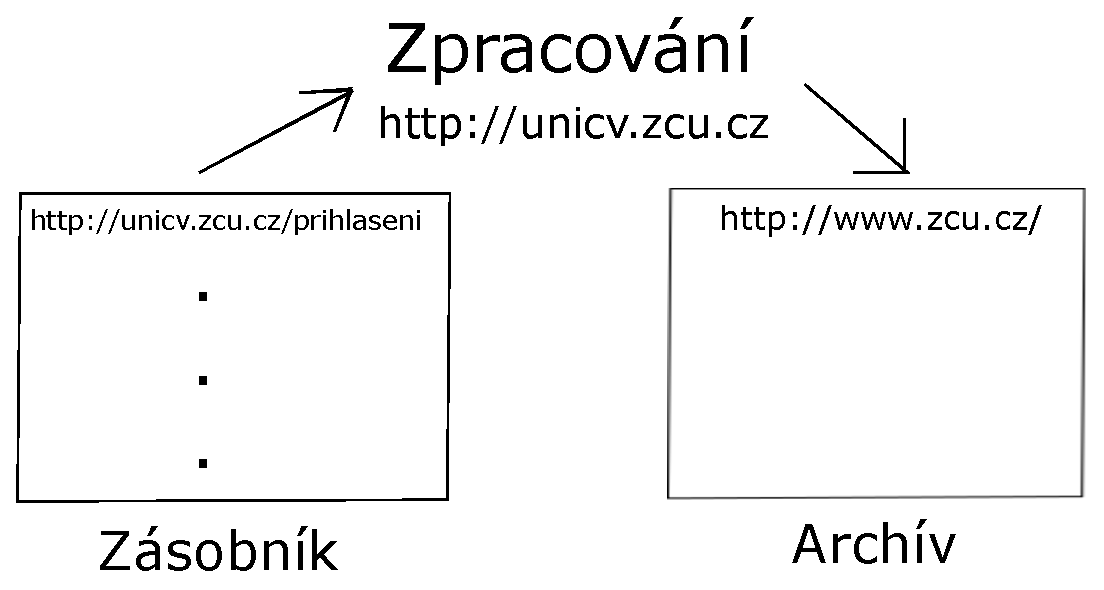
\includegraphics[width=250px]{stack_example.eps}}
\caption{Ukázka funkce zásobníku a archívu}
\label{obr.url_tree}
\end{figure}
Do zásobníku jsou ukládány instance třídy \textit{Parser::StackItem} (tato třída je pouze \uv{přepravka}\footnote{Třída, která slouží pouze k uchování dat.}), které mají 2 atributy: URL a hloubku zanoření. Před samotným spuštěním procházení je do zásobníku vložena kořenová stránka (v~našem případě \textit{http://unicv.zcu.cz}). Následně je spuštěn cyklus, který běží dokud zásobník není prázdný. Pokud stránku zpracujeme (včetně odkazů a formulářů), je uložena do pole historie. Každá nově přidávaná stránka \\do zásobníku je ověřována proti zásobníku i proti historii, aby nebyla jedna stránka procházena 2x.

\subsection{Získávání a uchovávání odkazů}
Při vytváření URL stromu webových stránek se ihned prochází načtené stránky a zjišťují se formuláře a odkazy na dané stránce. Pro uchování a následné zpracování se využívají 2 pomocné třídy:
\begin{itemize}
\item \textit{Parser::AContainer} - uchovává odkazy a parametry
\item \textit{Parser::FormContainer} - uchovává formuláře, metodu odesílání a jejich parametry
\end{itemize}
Při nalezení nového formuláře nebo odkazu jsou nejprve data porovnávána s poli ve třídě. Pokud již pole obsahuje formulář nebo odkaz, jsou tyto rozšiřovány, což je vidět u příkladu \ref{equals_classes2}, který ukazuje jednoduchost porovnání (za zmínku stojí i aliasování metod, které je řešeno takto: \textit{alias eql? ==}).

\begin{lstlisting}[label=equals_classes2,language=Ruby, caption=Porovnání dvou instancí třídy FormContainer]
# Equals method for comparing
# @param [FormContainer] another_form_container Another form container
# @return [boolean] True or false
def ==(another_form_container)
   # Action URL
   return @action != another_form_container.action && @type != another_form_container.type &&  @params != another_form_container.params
end

# Alias for ==
alias eql? ==
\end{lstlisting}

\subsection{Normalizace URL}
Na webové stránce máme relativně hodně možností jak zapisovat různé odkazy, od relativních cest \textit{./}, přes absolutní \textit{http://server.cz/index.php?action\\=nova}, až k pouhým \uv{skokům} na stránce \textit{$\#$novinky}. Veškeré tyto URL je potřeba normalizovat, ověřit server (pokud odkazy směřují mimo naší doménu, nejsou použity dále), získat data a odstranit nepotřebné části URL adresy. Při spuštění skriptu můžeme definovat \uv{wildcardování} domén, což znamená, že zadáme doménu prvního řádu: \textit{http://zcu.cz} a pokud je povoleno, bude skritp indexovat i domény vyšších řádů, například \textit{http://unicv.zcu.cz}. V následující tabulce je ukázka případů, kde kořenová doména je \textit{http://unicv.zcu.cz/}:

\begin{table}
\centering
\begin{tabular}{|l|l|}
\hline
\bf URL v odkazu & \bf Normalizovaná URL \\
\hline
\hline
./index.php?action=help &  http://unicv.zcu.cz/index.php?action=help \\
\hline
$\#$novinky & http://unicv.zcu.cz/$\#$novinky \\
\hline
unicv.zcu.cz/index.php?action=user & http://unicv.zcu.cz/index.php?action=user \\
\hline
http://www.seznam.cz/ & \bf Chybná URL - mimo zadaný server \\
\hline
\end{tabular}
\label{tab:url}
\caption{Příklady normalizování URL}
\end{table}
\newpage
Prvním krokem bylo nalezení již hotového řešení a výsledek byl překvapující. Ruby po provedení výchozí instalace obsahuje knihovnu \textit{uri}, která umožňuje požadované věci a umí s URL i velice snadno pracovat:

\begin{lstlisting}[label=equals_classes,language=Ruby, caption=Normalizování URL pomocí třídy URI]
# Spojeni 2 URL
url = URI.join("./index.php?action=help#fragment", "http://unicv.zcu.cz/") 
# http://unicv.zcu.cz/index.php?action=help#fragment

# Odstraneni fragmentu
url.fragment = nil
# http://unicv.zcu.cz/index.php?action=help

# Ziskani parametru
url.query
# {:action => "help"}
\end{lstlisting}


\section{Získání URL vectoru stránky}
Pro porovnání délky / obsahu stránek jsem vytvořil modul \textit{URLVector} (modul není třída), který má tři funkce:
\begin{enumerate}
\item Získání vektoru z HTML stránky
\item Odečtení dvou vektorů
\item Získání váhy vektoru
\end{enumerate}
URL vektor je běžná \textit{Hash}\footnote{Klíč - hodnota, v Ruby se klíči říká \textit{symbol}, který vždy začíná \uv{:}} struktura s pevně danými klíči, které jsou názvy elementů viz ukázka html stránky \ref{urlvector} a vektoru \ref{geturlvector} z ní získaného.
\begin{lstlisting}[label=urlvector,language=HTML, caption=HTML stránka]
<html>
   <head>
      <title>Music blog</title>
   </head>
   <body>
       <h1>My music blog</h1>
       <div class="song">
           <strong>Song name</strong>
             ...
       </div>
        ....
   </body>
</html>
\end{lstlisting}

\begin{lstlisting}[label=geturlvector,language=Ruby, caption=Získaný URL vektor]
url_vector = {
     :html => 1, :head => 1, :title => 1, 
     :body => 1, :h1 => 1, :div => 50, :strong => 50
}
\end{lstlisting}


\section{Testování se zapnutými chybovými direktivami pro PHP}
Testování se zapnutými chybovými direktivami je postaveno na principu, že se do parametrů postupně přidá uvozovka, která \uv{zničí} SQL dotaz, v tomto dotazu bude tudíž uvozovka navíc a tento dotaz se nepodaří provést a PHP preprocesor zahlásí chybu. Na stránce jsou tyto chyby následně vyhledávány:
\begin{itemize}
\item do verze PHP 5.2 - mysql$\_$error
\item od verze PHP 5.2 - php notice pro nesprávné použití \textit{while} (v konstrukcích iterací výsledky) nebo pro přístup k asociovaným polím, které neexistují.
\end{itemize}
Pokud je nějaká tato chyba na stránce nalezena, existuje zde vysoká pravděpodobnost, že se podařil SQL injection a tudíž byl SQL dotaz modifikován.

\section{Testování obsahu stránky při výměně parametrů}
Testování bez zapnutých direktiv není jednoznačné a výsledky je třeba ověřit ještě ručně. Pro porovnání výsledků s nahrazením parametrů se používají 3 možné případy:
\begin{enumerate}
\item \textit{'} - \uv{rozbití} SQL dotazu
\item \textit{' --} - zakomentování zbytku SQL příkazu
\item \textit{' OR '1' = '1} - logická pravda
\end{enumerate}

\subsection{Testování výsledků formulářů}
Formuláře se obecně používají na běžných webových stránkách ke 3 účelům:
\begin{enumerate}
\item Přihlašování
\item Vyhledávání 
\item Filtrování
\end{enumerate}
Pokud se \uv{podvodný} vstup dostane do dotazu, bude mít u každého typu formuláře jiný výsledek, proto se musí otestovat stránka jinak. Máme tudíž 4 webové stránky a vektor prvků na stránce. Vezmeme-li si možné situace, uvidíme, co se s vektory bude dít oproti bezchybnému průběhu. (Pozn. Body odpovídají výměně parametrů v sekci \textit{Testování a výměna parametrů})

\begin{itemize}
\item \textbf{Přihlašování}
\begin{enumerate}
\item Snížení počtu prvků na stránce, často přesměrování na nový formulář s hláškou, že chybný požadavek nelze zpracovat, protože SQL dotaz nebylo možno provést.
\item Velká změna při nahrazení v položce \uv{jména}. Díky zakomentování dotazu bude uživatel autorizován a bude přesměrován na stránku s jiným obsahem, zbytek SQL dotazu bylo zakomentováno popřípadě nastala logická pravda, tudíž vždy vrací výsledek.
\item To samé jako v bodě 2)
\end{enumerate}
\item \textbf{Vyhledávání a filtrování}
\begin{enumerate}
\item Snížením počtu prvků na 0 dotaz nevrátí žádný výsledek = snížení počtu elementů stránky.
\item Zvýšení počtu elementů, může být dosti zásadní (vypisují se všechny prvky) nebo menší (přibudou položky ve stránkování).
\end{enumerate}
\end{itemize}
Z výše zmíněného vyplývá, že je třeba určit všechny možnosti a určit příapady značnými rozdíly dle modelu chování, protože nejsme schopni strojově rozpoznat, jaký formulář testujeme.

\subsection{Testování výsledků odkazů}
Odkazy se testují na stejném principu jako formuláře, tj. hledají se změny obsahu pomocí vektoru elementů na stránce.

\section{Insert-into metoda}
Další možná metoda zjištění SQL injection, tato metoda vyžaduje předchozí zásah administrátora nebo vývojáře, je totiž nucen předem vytvořit tabulku \textit{sid\_log} (jejíž definice je uložena ve složce \textit{sql\_dump}). Po spuštění testu je do každého dotazu přidávána struktura \textit{'; INSERT INTO sid\_log(param) VALUE(param\_name)}. Tudíž pokud dotaz projde, je do tabulky přidáno jméno parametru, který tento vstup umožnil. Odpovědné osobě následně stačí tuto tabulku projít po dokončení testu.

\section{Drop-All metoda}
Do každého dotazu je přidána direktiva \textit{'; DROP ALL tables; ' --} nebo \textit{'; TRUNCATE ALL tables; ' --}, která způsobí vymazání všech tabulek. Pokud tento dotaz projde, změna obsahu bude skutečně zásadní, popřípadě bude zobrazena stránka 500 (služba je nedostupná). Tato metoda je \textit{opravdu destruktivní}, protože smaže opravdu vše.
